
\FloatBarrier
\subsection{Система Лоренца} % _LOR_

\LinkRef{
  lor: ASAU-22, 23, 24, 25, 26. APIR-2012. CSIT-2015. ISDMCI-2014, ISDMCI-2015.
  ITMM-2012, ITMM-2014, ITMM-2015, DSMP-2016
}

В качестве первой идентифицируемой хаотической системы рассмотрим
систему Лоренса, динамика которой описывается системой уравнений~[??]:

\begin{equation}
\begin{cases}
  \dot{x} = \sigma (y-x ) , \\
  \dot{y} = x (r-z) - y , \\
  \dot{z} = x y - b z .
\end{cases}
\label{atu:eq:lor}
\end{equation}

Наиболее ценным с точки зрения идентификации является параметр
$r$, определяющий как энергетическое состояние системы,
так и вид динамики системы.
Для определённости зададим остальные параметры следующим образом:
$b = 2.6666667$, $\sigma = 10$.

Критерий
$\overline{x^2}$


% Идентифицируемый параметр:
% $r \in [ 5; 100 ] $.
%
% Остальные параметры:
% $b = 2.66667$, $\sigma = 10$.


\begin{figure}[htb!]
\centerline{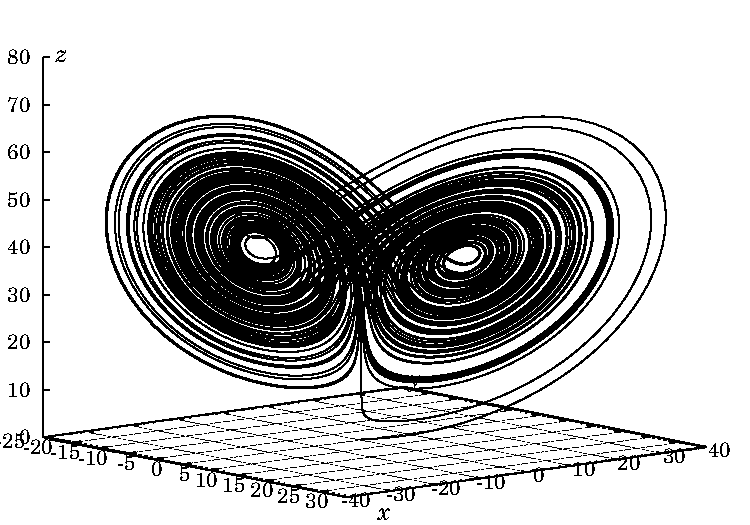
\includegraphics[width=0.5\textwidth]{p/cha/lor_phase3.pdf} }
\caption{Аттрактор системы Лоренца (\ref{atu:eq:lor})}
\label{atu:f:lor_phase}
\end{figure}


